% IEEE standard conference template; to be used with:
%   spconf.sty  - LaTeX style file, and
%   IEEEbib.bst - IEEE bibliography style file.
% --------------------------------------------------------------------------

\documentclass[letterpaper]{article}
\usepackage{spconf,amsmath,amssymb,graphicx,epstopdf,url,float}
\usepackage{algpseudocode} 
\usepackage{algorithm}
\usepackage{mathtools}

\algnewcommand\algorithmicforeach{\textbf{for each}}
\algdef{S}[FOR]{ForEach}[1]{\algorithmicforeach\ #1\ \algorithmicdo}

\algdef{S}[FOR]{ForEachParallel}[1]{\algorithmicforeach\ #1\ \algorithmicdo \textbf{\ parallel} }

\algnewcommand{\LineComment}[1]{\State \(\triangleright\) #1}

\algnewcommand\True{\textbf{true}\space}
\algnewcommand\False{\textbf{false}\space}
\algnewcommand\Continue{\textbf{continue}\space}

% Example definitions.
% --------------------
% nice symbols for real and complex numbers
\newcommand{\R}[0]{\mathbb{R}}
\newcommand{\C}[0]{\mathbb{C}}

% bold paragraph titles
\newcommand{\mypar}[1]{{\bf #1.}}

% Title.
% ------
\title{Maximum Cardinality Matching for Bipartite Graphs}
%
% Single address.
% ---------------
\name{Samuel Ueltschi, Conradin Roffler, Thomas Meier, Isabelle Roesch} 
\address{Department of Computer Science\\ ETH Z\"urich\\Z\"urich, Switzerland}

\begin{document}
%\ninept
%
\maketitle
%

%The hard page limit is 6 pages in this style. Do not reduce font size
%or use other tricks to squeeze. This pdf is formatted in the American letter format, so the spacing may look a bit strange when printed out.

\begin{abstract}
%Describe in concise words what you do, why you do it (not necessarily
%in this order), and the main result.  The abstract has to be
%self-contained and readable for a person in the general area. You
%should write the abstract last.
Maximum cardinality matching, focus on existing algorithms and optimize the parallel versions in a highly multi-threaded environment. Focus on Pothen-Fan, reason about performance.
\end{abstract}

\section{Introduction}\label{sec:intro}

\mypar{Motivation} Graph matching has several applications in computer science, for example the marriage problem or computing the block triangular form (BTF) of a sparse matrix \cite{Pothen:1990}. Bipartite graph matching is also a special case of a network flow problem. As data gets bigger, we are interested in the performance of the algorithms that solve these problems.

\mypar{Related work} Two parallel algorithms that we are testing on Xeon Phi \cite{Azad:2012} \cite{Azad:2015} 

%Do not start the introduction with the abstract or a slightly modified
%version. It follows a possible structure of the introduction. 
%Note that the structure can be modified, but the
%content should be the same. Introduction and abstract should fill at most the first page, better less.
%
%\mypar{Motivation} The first task is to motivate what you do.  You can
%start general and zoom in one the specific problem you consider.  In
%the process you should have explained to the reader: what you are doing,
%why you are doing, why it is important (order is usually reversed).
%
%For example, if my result is the fastest sorting implementation ever, one
%could roughly go as follows. First explain why sorting is important
%(used everywhere with a few examples) and why performance matters (large datasets,
%realtime). Then explain that fast implementations are very hard and
%expensive to get (memory hierarchy, vector, parallel). 
%
%Now you state what you do in this paper. In our example: 
%presenting a sorting implementation that is
%faster for some sizes as all the other ones.
%
%\mypar{Related work} Next, you have to give a brief overview of
%related work. For a report like this, anywhere between 2 and 8
%references. Briefly explain what they do. In the end contrast to what
%you do to make now precisely clear what your contribution is.

\section{Background: Algorithms for Maximum Matching in Bipartite Graphs}\label{sec:background}

\mypar{Maximum Matching}
Given a bipartite graph $G = (X \cup Y, E)$, where $V = X \cup Y$ are the vertices and $E$ the edges. The vertex set $V$ is partitioned into two disjoint subsets $X$ and $Y$ such that there are only edges between $X$ and $Y$. A matching $M$ in the graph is a subset of its edges such that no edge in $M$ shares a vertex with another edge in $M$. A matching $M$ in $G$ is \textit{maximal} if there is no other matching $M' \neq M$ such that $M \subset M'$. A maximal matching $M$ is a \textit{maximum} matching of the graph, if there is no other matching $M'$ such that $\lvert M' \rvert > \lvert M \rvert$. 

\mypar{State of the Art}
Best algorithms to solve this at the moment (parallel and sequential), as well as O(..) considerations

\mypar{Initial Matching}
Explain greedy matching, enhanced greedy matching (ours) and karp-siper initial matching.

%Give a short, self-contained summary of necessary
%background information. For example, assume you present an
%implementation of sorting algorithms. You could organize into sorting
%definition, algorithms considered, and asymptotic runtime statements. The goal of the
%background section is to make the paper self-contained for an audience
%as large as possible. As in every section
%you start with a very brief overview of the section. Here it could be as follows: In this section 
%we formally define the sorting problem we consider and introduce the algorithms we use
%including a cost analysis.
%
%\mypar{Sorting}
%Precisely define sorting problem you consider.
%
%\mypar{Sorting algorithms}
%Explain the algorithm you use including their costs.
%
%As an aside, don't talk about "the complexity of the algorithm.'' It's incorrect,
%problems have a complexity, not algorithms.


\section{Algorithms and Optimizations}\label{sec:pfopt}
%
%Now comes the ``beef'' of the report, where you explain what you
%did. Again, organize it in paragraphs with titles. As in every section
%you start with a very brief overview of the section.
%
%In this section, structure is very important so one can follow the technical content.
%
%Mention and cite any external resources that you used including libraries or other code.

Focus on Pothen-Fan \cite{Azad:2012} but also report Tree Grafting \cite{Azad:2015} for completeness

\subsection{Pothen-Fan}\label{sec:pf}
The work on the Pothen-Fan algorithm is the main part of our project. 
In this section we give a description of the algorithm based on \cite{Azad:2012} and present the
details of our implementation with a focus on the techniques we used to increase performance. In addition we also give a brief technical analysis of the theoretical complexity using the PRAM model.


\begin{algorithm}
    \caption{Parallel Pothen Fan}
    \begin{algorithmic}[1]
        \Procedure{PPF}{$G=(V=X+Y,E), M$}

        \LineComment{Initialization}
        \State $lookahead[x] \gets \text{first neighbor of x}$ \Comment{$x \in X$}
        \State $iter \gets 0$
        \State $visited[y] \gets iter$ \Comment{$y \in Y$}
        \State $unmatched \gets \{x \in X, x \ \text{unmatched}\}$

        \LineComment{Discover augmenting paths}
        \Repeat 
            \State $iter \gets iter + 1$        
            \State $path\_found \gets \False$        
        \ForEachParallel{$x \in unmatched$}
            \If {$x$ matched}
                \State \Continue \Comment{skip $x$ if already matched}
            \EndIf
            \State $found \gets find\_and\_augment(x)$        
            \If {found}
                \State $path\_found \gets \True$        
            \EndIf
        \EndFor
        \Until{$path\_found = \False$}

        \LineComment{Complete matching}
        \ForEachParallel{$y \in Y$, $y$ matched}
            \State $M[M[y] \gets y$        
        \EndFor
        
        \EndProcedure
    \end{algorithmic}
\end{algorithm}


\begin{algorithm}
    \caption{Find and Augment}
    \begin{algorithmic}[1]
        \Procedure{find\_and\_augment}{$x$}

            \LineComment{Lookahead Step}

            \ForEach{$y \in adj[x]$, starting at $lookahead[x]$}
                \State $lookahead[x] \gets \text{next neighbor of}\ x$
                \If {$y$ is unmatched}
                    \If {$claim(y)$}
                        \State $M[y] \gets x$ \Comment{make $x$ the mate of $y$}
                        \State \textbf{return} \True
                    \EndIf
                \EndIf
            \EndFor
            
            \LineComment{Recursive Path Search}
            \ForEach{$y \in adj[x]$}
                \If {$claim(y)$}
                    \State $success \gets find\_and\_augment(M[y])$
                    \If {$success$}
                        \State $M[y] \gets x$ \Comment{make $x$ the mate of $y$}
                        \State \textbf{return} \True
                    \EndIf
                \EndIf
            \EndFor
        \EndProcedure
    \end{algorithmic}
\end{algorithm}

\begin{algorithm}
    \caption{Claim with Test-and-Set}
    \begin{algorithmic}[1]
        \Procedure{$claim_{TAS}$}{$y$}
            \State $y\_iter \gets atomic\_exchange(visited[y], iter)$
            \State \textbf{return} $y\_iter < iter$
        \EndProcedure
    \end{algorithmic}
\end{algorithm}


\begin{algorithm}
    \caption{Claim with Test-and-Test-and-Set}
    \begin{algorithmic}[1]
        \Procedure{$claim_{TTAS}$}{$y$}
            \If {$visited[y] < iter$}
                \State $y\_iter \gets atomic\_exchange(visited[y], iter)$
                \State \textbf{return} $y\_iter < iter$
            \EndIf
            \State \textbf{return} \False
        \EndProcedure
    \end{algorithmic}
\end{algorithm}



\mypar{Parallel Pothen-Fan}
The original Pothen-Fan algorithm \cite{Pothen:1990} computes the maximum cardinality matching by finding augmenting paths. Azad et al. \cite{Azad:2012} presented a parallel version of Pothen-Fan where multiple augmenting paths can be found in parallel. 




\mypar{PRAM Analysis}
Show DAG, worst case O(n), best case O(1) with n processors (n nodes), but real world graph are rather O(1)

\mypar{Roofline Model}
number of operations, number of moves, what if whole graph fits into cache, etc

\mypar{Optimizations}
Test and Test and Set, Locality, Use only half of the visited array, set only half of the matching vector while setting the rest last, etc

\subsection{Tree Grafting}\label{sec:tg}

The second algorithm we examined that solves the problem of maximum matching on bipartite graphs is the Tree Grafting algorithm, as described in \cite{Azad:2015}. One of the paper's conclusions is that Tree Grafting performs better over Pothen-Fan on architectures with many thin cores, which the Xeon Phi essentially is. \\
We give a short overview of the algorithm we have implemented and on the optimizations we did.

\mypar{Parallel Tree Grafting} 
Parallel Tree Grafting (PTG) takes a bipartite graph and an initial matching $M $as input and returns a maximum matching by updating $M$.
PTG is - like Pothen-Fan - a multi-source searching algorithm. It starts to search for augmenting paths from different unmatched vertices and constructs a forest of alternating (matched-unmatched) trees.\\
The main difference to Pothen-Fan lies then in the reuse of already found trees. Pothen-Fan forgets about the trees it has previously found and starts again extending the augmenting paths with at most one vertex in every iteration. \\
PTG however keeps track of augmenting trees which can still be extended (active trees) and then grafts other trees to the active trees to prolong the augmenting paths contained in them.\\
For a more detailed explanation of the PTG algorithm including pseudocode, see \cite{Azad:2015}.\\
\mypar{Optimizations}
Our implementation of the PTG algorithm follows the implementation described in the paper very closely. To build the augmenting paths, we have used the same optimizations as already described in our best version of  PPF. To store the pointers to the root, leaf and other nodes the PTG algorithm utilizes, we have implemented our own version of a non-blocking queue as a data structure. 

\section{Experimental Results}\label{sec:exp}

%Here you evaluate your work using experiments. You start again with a
%very short summary of the section. The typical structure follows.

\mypar{Experimental setup} 
%Specify the platform (processor, frequency, maybe OS, maybe cache sizes)
%as well as the compiler, version, and flags used. If your work is about performance, 
%I strongly recommend that you play with optimization flags and consider also icc for additional potential speedup.

Xeon Phi (5110P), GCC, -O3, 60 simplified Intel CPU cores running at 1056 MHz and supports 4 threads per core, resulting in a total of 240 threads. Each core has a 32kb L1 data cache, a 32kb L1 instruction cache and a private 512 kb L2 unified cache. \cite{Ramos:2013}

%Then explain what kind of benchmarks you ran. The idea is to give enough information so the experiments are reproducible by somebody else on his or her code.
%For sorting you would talk about the input sizes. For a tool that performs NUMA optimization, you would specify the programs you ran.
\mypar{Test Data}
To test our algorithms, we have used several graphs from real-world examples. The graphs and their attributes are listed in \ref{table:testdata}. \\
\begin{table}
\centering
\begin{tabular}{ |l|l|l|l| }
\hline
 & $\lvert V \rvert$ & $\lvert E \rvert$ & Density \\ \hline
coPaperDBLP & 1'080'872 & 15'245'732 & $5.22\mathrm{e}{-5}$ \\ \hline
Wikipedia & 7'030'396 & 45'030'392 & $3.64\mathrm{e}{-6}$ \\ \hline
Amazon0312 & 801'454 & 3'200'440 & $1.99\mathrm{e}{-5}$ \\ \hline
Gnutella & 73'364 & 176'656 & $1.31\mathrm{e}{-4}$ \\ \hline
\end{tabular}
\caption{Test data used for benchmarks. $\lvert V \rvert$ is the number of vertices, $\lvert E \rvert$ the number of edges. The density describes the sparseness of the graph, where $0.0$ represents an empty graph and $1.0$ a fully connected bipartite graph.}
\label{table:testdata}
\end{table}
\mypar{Benchmarks}

Sequential Pothen-Fan

\mypar{Verification}

We use the \textit{Edmonds Maximum Cardinality Matching} algorithm \cite{BoostEdmonds} from the Boost Graph library  to verify the correctness of our implementations.

\mypar{Results}
%Next divide the experiments into classes, one paragraph for each. In each class of experiments you typically pursue one questions that then is answered by a suitable plot or plots. For example, first you may want to investigate the performance behavior with changing input size, then how your code compares to external benchmarks.
%
%For some tips on benchmarking including how to create a decent viewgraph see pages 22--27 in \cite{Pueschel:10}.

%{\bf Comments:}
%\begin{itemize}
%\item Create very readable, attractive plots (do 1 column, not 2 column plots
%for this report) with readable font size. However, the font size should also not be too large; typically it is smaller than the text font size.
%An example is in Fig.~\ref{fftperf} (of course you can have a different style).
%\item Every plot answers a question. You state this question and extract the
%answer from the plot in its discussion.
%\item Every plot should be referenced and discussed.
%\end{itemize}
%
%\begin{figure}\centering
%  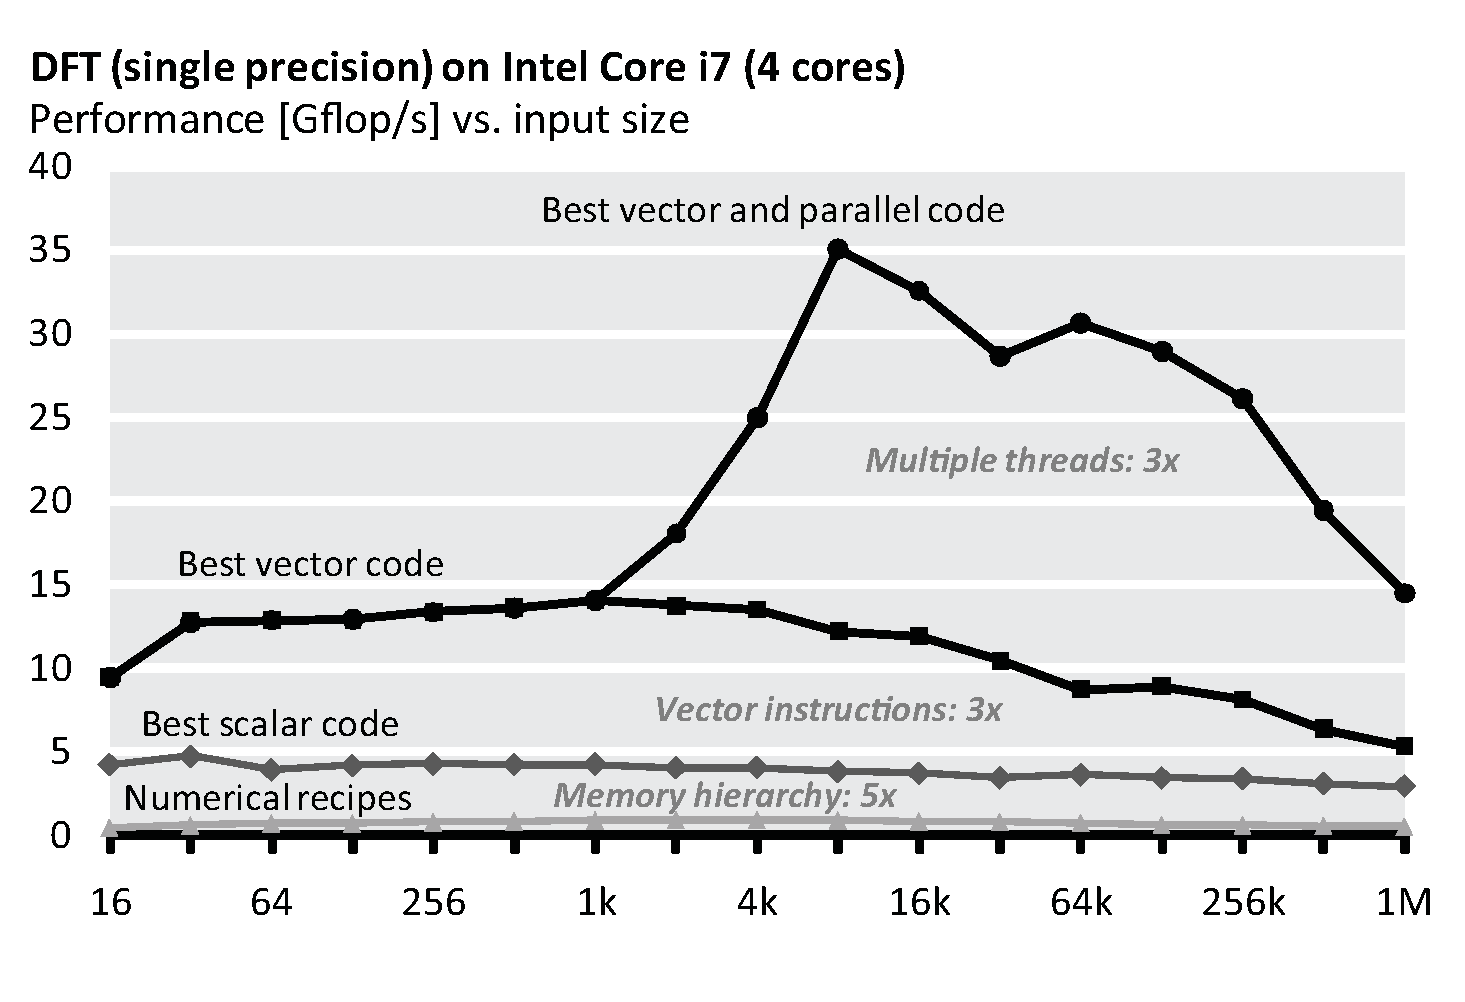
\includegraphics[scale=0.33]{dft-performance.eps}
%  \caption{Performance of four single precision implementations of the
%  discrete Fourier transform. The operations count is roughly the
%  same. The labels in this plot are maybe a little bit too small.\label{fftperf}}
%\end{figure}

\section{Conclusions}

Super linear speedup because of caching effects\\
PPF scales well on Xeon Phi\\
Tree Grafting results from the paper could not be reproduced.
%
%Here you need to summarize what you did and why this is
%important. {\em Do not take the abstract} and put it in the past
%tense. Remember, now the reader has (hopefully) read the report, so it
%is a very different situation from the abstract. Try to highlight
%important results and say the things you really want to get across
%such as high-level statements (e.g., we believe that .... is the right
%approach to .... Even though we only considered x, the
%.... technique should be applicable ....) You can also formulate next
%steps if you want. Be brief. After the conclusions there are only the references.
%
%\section{Further comments}
%
%Here we provide some further tips.
%
%\mypar{Further general guidelines}
%
%\begin{itemize}
%\item For short papers, to save space, I use paragraph titles instead of
%subsections, as shown in the introduction.
%
%\item It is generally a good idea to break sections into such smaller
%units for readability and since it helps you to (visually) structure the story.
%
%\item The above section titles should be adapted to more precisely
%reflect what you do.
%
%\item Each section should be started with a very
%short summary of what the reader can expect in this section. Nothing
%more awkward as when the story starts and one does not know what the direction is or the goal.
%
%\item Make sure you define every acronym you use, no matter how
%convinced you are the reader knows it.
%
%\item Always spell-check before you submit (to us in this case).
%
%\item Be picky. When writing a paper you should always strive for very
%high quality. Many people may read it and the quality makes a big difference.
%In this class, the quality is part of the grade.
%
%\item Books helping you to write better: \cite{Higham:98} and \cite{Strunk:00}.
%
%\item Conversion to pdf (latex users only): 
%
%dvips -o conference.ps -t letter -Ppdf -G0 conference.dvi
%
%and then
%
%ps2pdf conference.ps
%\end{itemize}

%\mypar{Graphics} For plots that are not images {\em never} generate the bitmap formats
%jpeg, gif, bmp, tif. Use eps, which means encapsulate postscript. It is
%scalable since it is a vector graphic description of your graph. E.g.,
%from Matlab, you can export to eps.
%
%The format pdf is also fine for plots (you need pdflatex then), but only if the plot was never before in the format 
%jpeg, gif, bmp, tif.


% References should be produced using the bibtex program from suitable
% BiBTeX files (here: bibl_conf). The IEEEbib.bst bibliography
% style file from IEEE produces unsorted bibliography list.
% -------------------------------------------------------------------------
\bibliographystyle{IEEEbib}
\bibliography{bibl_conf}

\end{document}

